\documentclass{udparticle}
\headertext{Metodos Numéricos}
\title{Metodos Numéricos : Tarea 1}
\author{Thomas Muñoz , Diego Vilches , Javiera Araya , Ignacio Yanjari.}
\usepackage{amssymb}
\usepackage{amsmath}
\usepackage{graphicx}
\usepackage{float}
\usepackage{array}
\graphicspath{ {images/} }

\begin{document}
\maketitle
\section{Resolución de sistemas de ecuaciones no lineales:}
\begin{enumerate}
\item Usando los métodos de bisección, falsa posición, y secante, encuentre la raíz aproximada 
de las siguientes ecuaciones no lineales en los intervalos indicados:

\begin{enumerate}
    
Para realizar estas ecuaciones se utilizaron los programas de :
\begin{itemize}
    \item Biseccion.m
    \item Secante.m
    \item FalsaPosicion.m
\end{itemize}
y las comparaciones de error se hicieron en base a el resultado de la función fzero de matlab

\item  \(x^3 - 3sen(x) +1 = 0\) , sobre [0,2].
\begin{figure}[H]
    \centering
    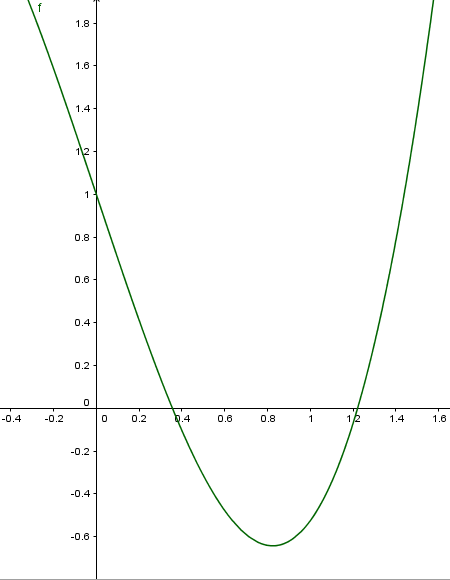
\includegraphics[width=9cm]{GraficoEj1a}
\end{figure}
Nuestro objetivo es obtener el 0 de la función para resolver la ecuacion lineal, pero esta como muestra el gráfico tiene 2 soluciones.Para lograr analizar completamente estos 2 casos con los 3 métodos diferentes tendremos que separar en 2 intervalos nuestro intervalo anterior, en este caso lo separaremos en [0,0.8] y [0.8,2]\\
    \begin{table}[H]Intervalo [0,0.8]:
    \centering
        \begin{tabular} { |c|c|c|c|}
        \hline
        Métodos       & Secante & Biseccion & Falsa Posicion  \\
        \hline
        Cero Obtenido &  0,3558       &    0,3558       &      0,3558    \\
        \hline
        Iteraciones   &     5        &      13     &        5          \\
        \hline
        Error Obtenido &       0      &       0      &     0         \\
         \hline
        \end{tabular}
    \end{table}

    \begin{table}[H]Intervalo [0.8,2]:
    \centering
        \begin{tabular} { |c|c|c|c|}
            \hline
            Métodos       & Secante & Biseccion & Falsa Posicion  \\
            \hline
        Cero Obtenido &  1.2204       &    1.2204       &      1.2204    \\
        \hline
        Iteraciones   &     8       &      11     &        19          \\
        \hline
        Error Obtenido &    0         &      0       &      0        \\
         \hline
        \end{tabular}
    \end{table}

    
\item \( e^{-t/2} cos(4t) = 0 \), sobre [0,1].

    \begin{figure}[H]
        \centering
        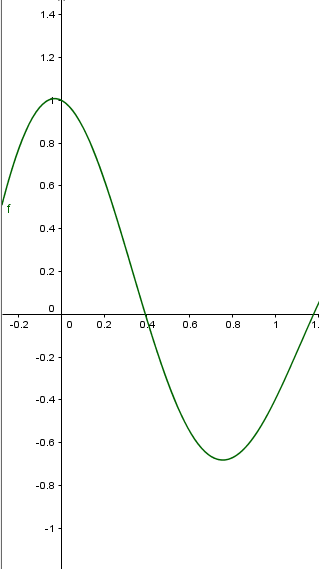
\includegraphics[width=8cm]{GraficoEj1b}
    \end{figure}
    
    \begin{table}[H]
    \centering
        \begin{tabular} { |c|c|c|c|}
        
        \hline
        Métodos       & Secante & Biseccion & Falsa Posicion \\
        \hline
        Cero Obtenido &  1,9635       &    0,3927       &      0,3927           \\
        \hline
        Iteraciones   &     3        &      12     &        4         \\
        \hline
        Error Obtenido &     4      &     0        &    0  \\
        \hline
        
        \end{tabular}
    \end{table}
    Como se observa en la tabla el valor obtenido por el método de la secante es muy diferente al cero 
    obtenido por los otros 2 que son Biseccion y falsa posición,los cuales encuentran el cero contenido en el intervalo pedido.Esto se debe a la forma en la cual se desarrolla el método de secante, el cual no usa un criterio entre 2 intervalos para encontrar el cero, para obtener el cero correcto se debe definir como [0-0.8] y se encuentra el cero de 0,3927    
    
\newpage
    
    

\item \(x + 40 -x\cosh(\frac{60}{x}) = 0 \), sobre [40,60].\\
\begin{figure}[H]
    \centering
    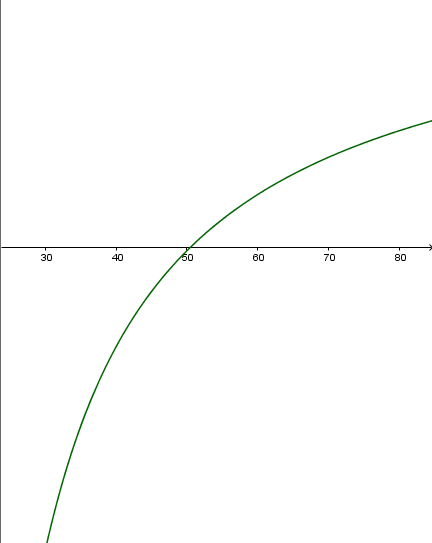
\includegraphics[width=10cm]{GraficoEj1c}
\end{figure}
    \begin{table}[H]
    \centering
        \begin{tabular} { |c|c|c|c|}
        
        \hline
        Métodos       & Secante & Biseccion & Falsa Posicion  \\
        \hline
        Cero Obtenido &  50,5399       &    50,5399       &      50,5399          \\
        \hline
        Iteraciones   &     5        &      15     &        9        \\
        \hline
        Error Obtenido &    0       &       0       &       0   \\
        \hline 
        
        \end{tabular}
    \end{table}
\newpage

\item \(e^{0.5x}\cos(0.05\sqrt{200-\frac{x^2}{10}}) -1 = 0 \), sobre [0,4].\\
    
    \begin{figure}[H]
    \centering
    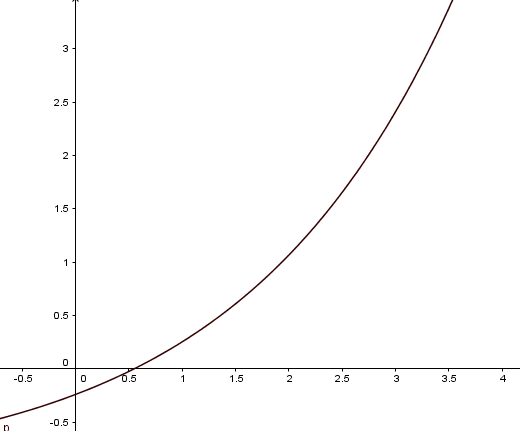
\includegraphics[width=10cm]{GraficoEj1d}
    \end{figure}
    \begin{table}[H]
    \centering
        \begin{tabular} { |c|c|c|c|}
        
        \hline
        Métodos       & Secante & Biseccion & Falsa Posicion \\
        \hline
        Cero Obtenido &  0.5481       &    0.5481       &      0.5481          \\
        \hline
        Iteraciones   &     5        &      13     &        18       \\
        \hline
        Error Obtenido   &  0 & 0 & 0 \\
        \hline
        
        \end{tabular}
    \end{table}
\newpage
\item $ f (\theta) = \frac{0.6\sen{\theta}}{\sqrt{(cos(\theta) - 0.6)^2 + sen(\theta)^2}} -  \frac{0.6\sen{\theta}}{\sqrt{(cos(\theta) + 0.6)^2 + sen(\theta)^2}} = 0, \theta \in [1,2].$
$(sol. exacta \theta^* = \frac{\pi}{2})$

    \begin{figure}[H]
    \centering
    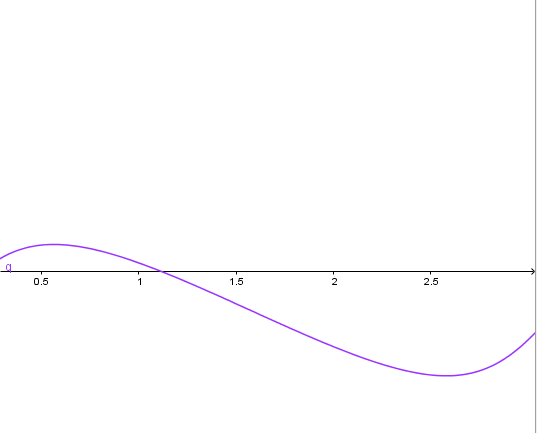
\includegraphics[width=11cm]{GraficoEj1e}
    \end{figure}

    \begin{table}[H]
    \centering
        \begin{tabular} { |c|c|c|c|}
        
        \hline
        Métodos       & Secante & Biseccion & Falsa Posicion \\
        \hline
        Cero Obtenido &  1,5708       &   1,5708       &      1,5708        \\
        \hline
        Iteraciones   &     3        &      10        &        2       \\
        \hline
        Error Obtenido  &   0        &      0      &          0  \\
        \hline
        
        \end{tabular}
    \end{table}
    
Con una tolerancia de $ 10^{-5} $. Haga una comparación de los métodos en cuanto a la cantidad de iteraciones, el error cometido. Cuál de ellos fue más eficiente?

El metodo más eficiente para lograr encontrar el valor de las funciones mencionadas es el metodo de Falsa Posicion ya que encontró el cero en todas las ecuaciones y necesitó en promedio un menor número de iteraciones en comparación con Bisección.Pero si no le damos importancia a la convergencia en el caso b) el mejor y más rapido sería el método de secante.

\end{enumerate}
\newpage
\item %pregunta 2
\newpage
%pendiente: poner gráfica
\item Considere la ecuación no lineal $f(x)= \frac{1}{2}+\frac{1}{4}x^2-xsen(x)-\frac{1}{2}cos(2x)=0$
	\begin{enumerate}
	\item  Usando el método de Newton con punto inicial $x_{0}=\frac{\pi}{2}$ encuentre la solución aproximada de $f$. Para ello REalize las iteraciones necesarias hasta que se cumpla el criterio de parada %$\abs{x_{n+1}-x_{n}} \l 10^{-6} $

%pregunta 2
%pendiente: poner gráfica
\item Considere la ecuación no lineal $f(x)= \frac{1}{2}+\frac{1}{4}x^2-xsen(x)-\frac{1}{2}cos(2x)=0$
	\begin{enumerate}
	\item  Usando el método de Newton con punto inicial $x_{0}=\frac{\pi}{2}$ encuentre la solución aproximada de $f$. Para ello REalize las iteraciones necesarias hasta que se cumpla el criterio de parada $|x_{n+1}-x_{n}| < 10^{-6} $
%pendiente: valor absoluto

		\begin{table} [H]
			\centering
			\begin{tabular}{|c|c|c|}
				\hline
				$x_{0}$ & Cero Obtenido & Iteraciones\\
				\hline
				$\frac{\pi}{2} $ & 1,8955 & 18\\
				\hline 
			\end{tabular}
		\end{table}
	
	\item Repita el proceso tomando como valores iniciales $x_{0}=5\pi$ y $x_{0}=10\pi$ ¿La sucesión construída con estos puntos iniciales converge?
	 	\begin{table} [H]
			\centering
			\begin{tabular}{|c|c|c|}
				\hline
				$x_{0}$ & Cero Obtenido & Iteraciones\\
				\hline
				$5\pi$ & 1,8955 & 22 \\
				\hline 
				$10\pi$ & 0 & 66\\
				\hline
			\end{tabular}
		\end{table}
		
La sucesión, en el caso de $x_{0}=5\pi$, converge al mismo cero que en el ejercicio anterior. Por otra parte, cuando $x_{0}=10\pi$, esta converge a 0.

	\item Use el método de la secante para encontrar la solución aproximada tomando como puntos iniciales $x_{0}=\frac{\pi}{2}$ y $x_{0}=5\pi$, como criterio de parada el mismo descrito en (a).
	\begin{table} [H]
			\centering
			\begin{tabular}{|c|c|c|c|}
				\hline
				$x_{0}$& $x_{1}$ & Cero Obtenido & Iteraciones\\
				\hline
				$\frac{\pi}{2}$ & 1,7854 & 1,8955 & 24 \\
				\hline 
				$5\pi$& 13,0900 & 0 & 31\\
				\hline
			\end{tabular}
		\end{table}
		
Se puede apreciar que si $x_{0}=5\pi$, al ocupar el método de la secantem se obtiene un cero distinto a cuando se ocupa el método de Newton.	
	\end{enumerate}
		

\item Considere la ecuación no lineal $f(x) = -x^{3} - \cos(x) = 0$
    \begin{enumerate}
    
        \item Usando el método de Newton encontrar la raíz próxima al valor $x_{0}=-1$, con una precisión de $10^{-5}$.\\
        \begin{table}[H]
        \centering
        \begin{tabular} { |c|c|}
        
        \hline
        Cero Obtenido &  -0.8655\\
        \hline
        Iteraciones   &    4\\
        \hline
        
        \end{tabular}
        \end{table}
        
        \item Repetir el proceso con el método de Newton modificado, esto es, con la iteración $$x_{n+1} = x_{n} - \frac {f(x_{n})} {f'(x_{0})} $$
        \begin{table}[H]
        \centering
        \begin{tabular} { |c|c|}
        
        \hline
        Cero Obtenido &  -0.8655\\
        \hline
        Iteraciones   &    7\\
        \hline
        
        \end{tabular}
        \end{table}
        ¿Qué método converge más rápido?
        El método de Newton usual converge más rápido, ya que solo tomó 4 iteraciones %debo graficar y argumentar.
    \end{enumerate}
\end{enumerate}
\newpage
\item El dinero necesario para pagar la cuota correspondiente a un crédito hipotecario a interés fijo se suele
estimar mediante la denominada “ecuación de la anualidad ordinaria”:
\begin{center}
    $ Q = \frac{A}{i}(1-(1+i)^{-n}) $
\end{center}
donde Q es la cantidad pedida en préstamo, A es la cuota que debe pagar el beneficiario por el
préstamo, i es la tasa de interés fijado por la entidad bancaria que concede el préstamo y n es el
número de periodos durante los cuales se realizan pagos de la cuota.
Una pareja que desea comenzar una vida en común se plantea adquirir una vivienda y para ello saben
que necesitan pedir un préstamo de 15000 dólares a pagar semestralmente durante un plazo de 10 años.
Sabiendo que para atender este pago pueden destinar una cantidad máxima de 200 dólares mensuales,
calcule cual es el tipo máximo de interés al que pueden negociar su préstamo con las entidades bancarias.
Hint.- Usar método de Newton, tomando como punto inicial i0 = 0.03.
Suponga ahora que desean endeudarse en 15 años en lugar de 10. Cual sería el interés en esta situación?


\item Considere la función \(f(x) = x*cos(x)-e^x+ 1\). % pregunta 5 
\begin{enumerate}
    
\vspace{0.9cm}
\item Considere las siguientes funciones. Realice unas 12 iteraciones de punto fijo, usando como puntos iniciales x0 = 0.5 y x0 = 0.5.\\ 


\begin{equation}
 g1(x) = \frac{e^x+x-1}
{1 + cos(x)}
\end{equation}
\\
\begin{itemize}
\item x0=0.5
\end{itemize}


\begin{table}[H]
    \centering
        \begin{tabular} { |c|c|}
        
        \hline
        iteración  &  Punto\\
        \hline
        1 &  0,6118        \\
         \hline
        2 &  0,8004        \\
         \hline
        3 &  1,1947        \\
         \hline
        4 &  2,5579        \\
         \hline
        5 &  87,3616        \\
         \hline
        6 & 4,7832e+37        \\
         \hline
        7 & inf           \\
         \hline
        8 &  NaN        \\
         \hline
        9 &  NaN        \\
         \hline
        10 &  NaN        \\
         \hline
        11 &  NaN        \\
         \hline
        12 &  NaN        \\
        \hline
        
        \end{tabular}
    \end{table}
 
 \begin{itemize}
 \newpage
\item x0=-0.5
\end{itemize}
\begin{table}[H]
    \centering
        \begin{tabular} { |c|c|}
        
        \hline
        iteración  &  Punto\\
        \hline
        1 &  -0.4759        \\
         \hline
        2 &  -0.4524        \\
         \hline
        3 &  -0.4298        \\
         \hline
        4 &   -0.4081      \\
         \hline
        5 &  -0.3875        \\
         \hline
        6 &  -0.3680       \\
         \hline
        7 &  -0.3497        \\
         \hline
        8 &  -0.3324        \\
         \hline
        9 &  -0.3163        \\
         \hline
        10 &  -0.3012       \\
         \hline
        11 &  -0.2871       \\
         \hline
        12 &  -0.2739        \\
        \hline
        \end{tabular}
\end{table}

\begin{equation}
 g2(x) = \frac{\sqrt{x(e^x-1)}}
{cos(x)}
\end{equation}
\\
\begin{itemize}
\item x0=0.5
\end{itemize}

\begin{table}[H]
    \centering
        \begin{tabular} { |c|c|}
        
        \hline
        iteración  &  Punto\\
        \hline
        1 &  0.6080       \\
         \hline
        2 &   0.7872     \\
         \hline
        3 &  1.1555       \\
         \hline
        4 &   2.4964     \\
         \hline
        5 & 0.0000 + 5.8994i        \\
         \hline
        6 &  0.1106 - 0.0106i       \\
         \hline
        7 & 0.1140 - 0.0113i         \\
         \hline
        8 &    0.1177 - 0.0121i     \\
         \hline
        9 &     0.1216 - 0.0130i     \\
         \hline
        10 &   0.1258 - 0.0140i       \\
         \hline
        11 &    0.1303 - 0.0151i   \\
         \hline
        12 &  0.1351 - 0.0163i        \\
        \hline
        
        \end{tabular}
        
    \end{table}
    \begin{itemize}
\item x0=-0.5
\end{itemize}

\begin{table}[H]
    \centering
        \begin{tabular} { |c|c|}
        
        \hline
        iteración  &  Punto\\
        \hline
        1 &  0.4735       \\
         \hline
        2 &   0.5676     \\
         \hline
        3 &  0.7171
       \\
         \hline
        4 &   0.9989     \\
         \hline
        5 & 1.7791        \\
         \hline
        6 &  0.0000 + 6.5089i      \\
         \hline
        7 &   0.0037 - 0.0660i       \\
         \hline
        8 &     0.0026 - 0.0660i   \\
         \hline
        9 &   0.0015 - 0.0660i       \\
         \hline
        10 &    0.0004 - 0.0660i      \\
         \hline
        11 &    0.0007 + 0.0659i \\
         \hline
        12 &   0.0004 - 0.0659i       \\
        \hline
        
        \end{tabular}
        
    \end{table}
 \vspace{3cm}   
 \item Teniendo en cuenta las siguientes funciones de iteración de punto fijo.  Realize unas 12 iteraciones de punto fijo, usando como puntos iniciales x0 = 0.5 y x0 = 0.5.\\   
 
 \begin{equation}
 g3(x) = x-\frac{f(x)}
{f'(x)}
\end{equation}
\\
 \begin{itemize}
\item x0=0.5
\end{itemize}

\begin{table}[H]
    \centering
        \begin{tabular} { |c|c|}
        
        \hline
        iteración  &  Punto\\
        \hline
        1 &   0.2923       \\
         \hline
        2 &     0.1645   \\
         \hline
        3 &  0.0891 \\
         \hline
        4 &  0.0468     \\
         \hline
        5 &    0.0241    \\
         \hline
        6 & 0.0122       \\
         \hline
        7 &    0.0062 \\
         \hline
        8 &  0.0031     \\
         \hline
        9 &      0.0015    \\
         \hline
        10 &    7.7566e-04     \\
         \hline
        11 &   3.8803e-04  \\
         \hline
        12 &   1.9407e-04      \\
        \hline
        
        \end{tabular}
        
    \end{table}
 \begin{itemize}
\item x0=-0.5
\end{itemize}

\begin{table}[H]
    \centering
        \begin{tabular} { |c|c|}
        
        \hline
        iteración  &  Punto\\
        \hline
        1 &  0.9462        \\
         \hline
        2 &     0.5755  \\
         \hline
        3 &    0.3398        \\
 
         \hline
        4 &   0.1932  \\
         \hline
        5 &  0.1057       \\
         \hline
        6 &      0.0560  \\
         \hline
        7 & 0.0289    \\
         \hline
        8 & 0.0147      \\
         \hline
        9 &   0.0074       \\
         \hline
        10 &    0.0037     \\
         \hline
        11 &   0.0019  \\
         \hline
        12 &   9.3724e-04     \\
        \hline
        
        \end{tabular}
        
    \end{table}
 \vspace{2cm}
     \begin{equation}
 g4(x) = x-2\frac{f(x)}
{f'(x)}
\end{equation}
\newpage
 \begin{itemize}
\item x0=0.5
\end{itemize}

\begin{table}[H]
    \centering
        \begin{tabular} { |c|c|}
        
        \hline
        iteración  &  Punto\\
        \hline
        1 &      0.0846   \\
         \hline
        2 &    0.0041    \\
         \hline
        3 &   1.1230e-05 \\
         \hline
        4 &   8.4146e-11    \\
         \hline
        5 &   8.4146e-11   \\
         \hline
        6 &   8.4146e-11     \\
         \hline
        7 & 8.4146e-11   \\
         \hline
        8 &  8.4146e-11   \\
         \hline
        9 &   8.4146e-11      \\
         \hline
        10 &   8.4146e-11      \\
         \hline
        11 & 8.4146e-11   \\
         \hline
        12 &  8.4146e-11      \\
        \hline
        
        \end{tabular}
        
    \end{table}
     \begin{itemize}
\item x0=-0.5
\end{itemize}

\begin{table}[H]
    \centering
        \begin{tabular} { |c|c|}
        
        \hline
        iteración  &  Punto\\
        \hline
        1 &     2.3924  \\
         \hline
        2 &    0.6344   \\
         \hline
        3 &   0.1196 \\
         \hline
        4 &    0.0078   \\
         \hline
        5 &   3.9737e-05  \\
         \hline
        6 &   1.0509e-09    \\
         \hline
        7 & 1.0509e-09   \\
         \hline
        8 &  1.0509e-09  \\
         \hline
        9 &  1.0509e-09      \\
         \hline
        10 &  1.0509e-09      \\
         \hline
        11 & 1.0509e-09   \\
         \hline
        12 &  1.0509e-09     \\
        \hline
        
        \end{tabular}
        
    \end{table}
    \vspace{3cm}
    \begin{equation}
 g5(x) = x-\frac{f(x)f'(x)}
{(f'(x))^2-f(x)f''(x)}
\end{equation}
\\
 \begin{itemize}
 \newpage
\item x0=0.5
\end{itemize}
\begin{table}[H]
    \centering
        \begin{tabular} { |c|c|}
        
        \hline
        iteración  &  Punto\\
        \hline
        1 &  -0.0551      \\
         \hline
        2 &    -0.0023   \\
         \hline
        3 &  -3.5887e-06 \\
         \hline
        4 &  1.2916e-10    \\
         \hline
        5 &    1.2916e-10  \\
         \hline
        6 &  1.2916e-10     \\
         \hline
        7 &     1.2916e-10 \\
         \hline
        8 &  1.2916e-10    \\
         \hline
        9 &       1.2916e-10   \\
         \hline
        10 &    1.2916e-10     \\
         \hline
        11 &    1.2916e-10 \\
         \hline
        12 &   1.2916e-10  \\
        \hline
        
        \end{tabular}
        
    \end{table}
     \begin{itemize}
\item x0=0.5
\end{itemize}
\begin{table}[H]
    \centering
        \begin{tabular} { |c|c|}
        \hline
        iteración  &  Punto\\
        \hline
        1 &  -0.4614      \\
         \hline
        2 &   -0.3825   \\
         \hline
        3 &  -0.2366 \\
         \hline
        4 &  -0.0667    \\
         \hline
        5 &   -0.0035 \\
         \hline
        6 & -8.1704e-06     \\
         \hline
        7 &     -2.6231e-11 \\
         \hline
        8 &   -2.6231e-11   \\
         \hline
        9 &        -2.6231e-11 \\
         \hline
        10 &     -2.6231e-11    \\
         \hline
        11 &    -2.6231e-11 \\
         \hline
        12 &    -2.6231e-11  \\
        \hline
        \end{tabular}
    \end{table}
\vspace{3cm}
\item Que puede decir sobre el comportamiento de las iteraciones de punto fijo calculadas anteriormente.
\begin{itemize}

\item De la función g1(x), cuando se toma el punto inicial x0=0.5, la iteración por punto fijo diverge, pues, cada vez que se hacen más iteraciones, el punto fijo tendera a infinito. 
\end{itemize}

\end{enumerate}
<<<<<<< HEAD
\item Según los metodos descritos(Nweton, Schröder y Whittaker) para encontrar la raíz aproximada de $f(x)=0$:
=======
\newpage
\item Métodos iterativos :A continuación se describen algunos métodos de iteración de punto fijo que encuentran la raíz aproximada de f(x) = 0
\begin{itemize}
        \item Método de Newton     
            \begin{equation*}
                 x_{n+1}=N_f(x_n)=x_n -  \frac{f(x_n)}{f^{'}(x_n)}
            \end{equation*}
        
        \item Método de Schröder
            \begin{equation*}
                x_{n+1}=S_f(x_n)=x_n-\frac{f(x_n)f^{'}(x_n)}{f^{'}(x_n)^{2}-f(x_n)f^{''}(x_n)}
            \end{equation*}
        
        \item Método de aceleración convexa de Whittaker
            \begin{equation*}
                x_{n+1}=W_f(x_n)=x_n - \frac{f(x_n)}{2f^{'}(x_n)}(2 - L_f(x_n))
            \end{equation*}
        
\end{itemize}
>>>>>>> 2d15196d83295c79463f3c1fbf4094e856e2e603
	\begin{enumerate}
	
		\item Utilize los métodos para encontrar la solución de la ecuación no lineal $f(x)=0$, donde
		
		(i) $f_{1}(x)=xe^{x^2}-sen(x)+3cos(x)+5$.
		
		\begin{table}[H]
			\centering
			\begin{tabular}{|c|c|c|c|}
				\hline
				Métodos & $x_{0}$ & Iteraciones & Cero Obtenido \\
				\hline
				Newton & -1 & 6 & -1.2892 \\
				\hline
				Schroder & -1 & 6 & -1.2892 \\
				\hline
				Whittaker & -1 & 10 & -1.2892 \\
				\hline				
			\end{tabular}
			\end{table}	
		
		
		
		(ii) $f_{2}(x)=x^3-3x^2(2^{-x})+3x(4^{-x})-8^{-x}$, en [0,1].
		
			\begin{table}[H]
			\centering
			\begin{tabular}{|c|c|c|c|}
				\hline
				Métodos & $x_{0}$ & Iteraciones & Cero Obtenido \\
				\hline
				Newton & 1 & 43 & 0.6412 \\
				\hline
				Schroder & 1 & 4 & 0.6412\\
				\hline
				Whittaker & 1 & 66 & 0.6412\\
				\hline				
			\end{tabular}
			\end{table}	
			
		(iii) $f_{3}(x)=cos(x+\sqrt[2]{2})+x(\frac{x}{2}+2)$, en [-2,1].	
		
		\begin{table}[H]
			\centering
			\begin{tabular}{|c|c|c|c|}
				\hline
				Métodos & $x_{0}$ & Iteraciones & Cero Obtenido \\
				\hline
				Newton & -1 & 5 & -0.1646 \\
				\hline
				Schroder & -1 & 5 & -0.1646\\
				\hline
				Whittaker & -1 & 6 & -0.1646 \\
				\hline				
			\end{tabular}
		\end{table}		
			
		\item Compare los errores relativos vs. las iteraciones (mediante un gráfico) para los métodos (descritos
			anteriormente) que determinan la raíz de $f_{i}(x)=0$, para $i$ = 1,2,3.	
			\begin{itemize}
				\item Método de Newton:
				\begin{figure}[H]
					\centering
<<<<<<< HEAD
					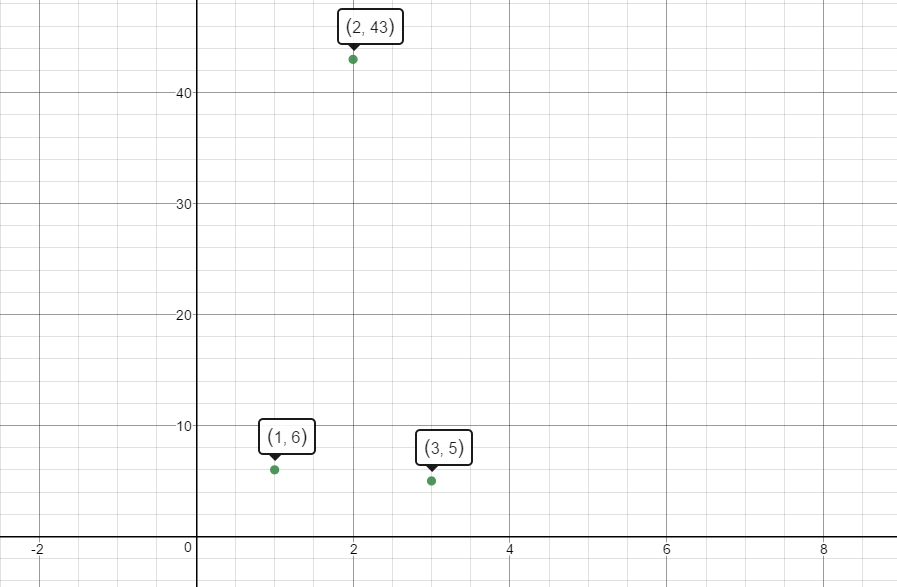
\includegraphics[width=10cm]{NewtonEj6} 
				\end{figure}								 
				
				
				\item Métdo de Schröder: 
				 \begin{figure}[H]
					\centering
					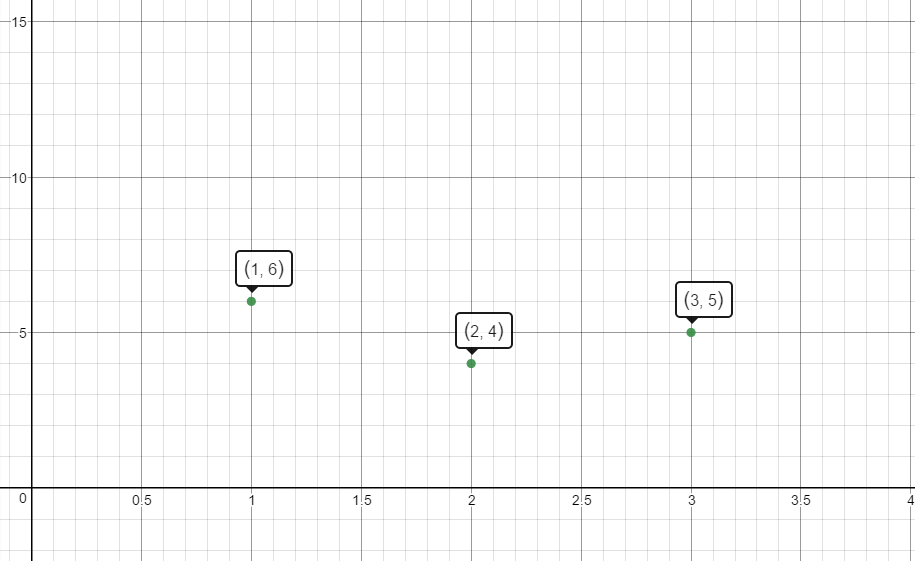
\includegraphics[width=10cm]{SchroderEj6} 
				\end{figure}	
				 
				 
				 \item Método de Whittaker;
				 \begin{figure}[H]
					\centering
					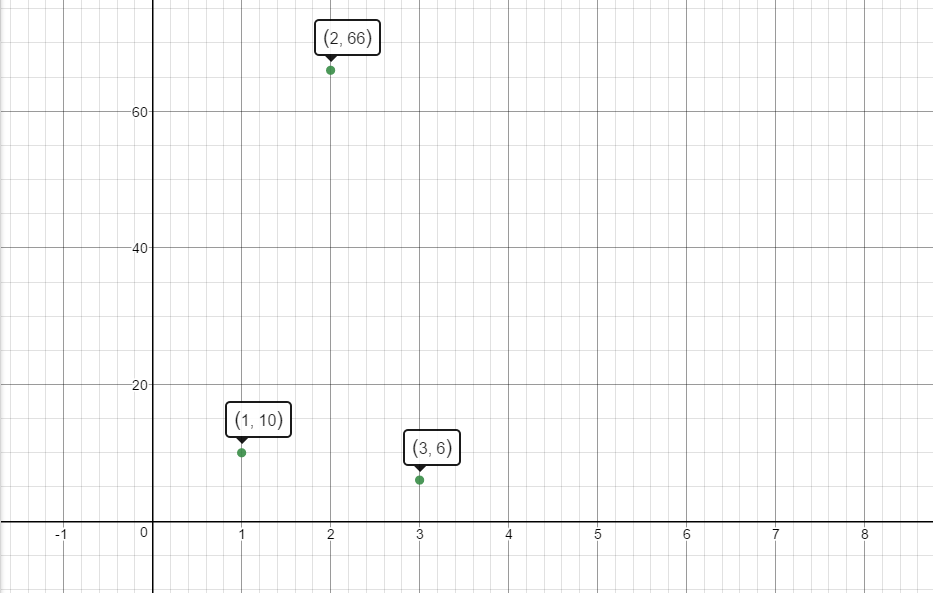
\includegraphics[width=10cm]{WhittakerEj6} 
				\end{figure}	
			\end{itemize}				
		
	
	
=======
					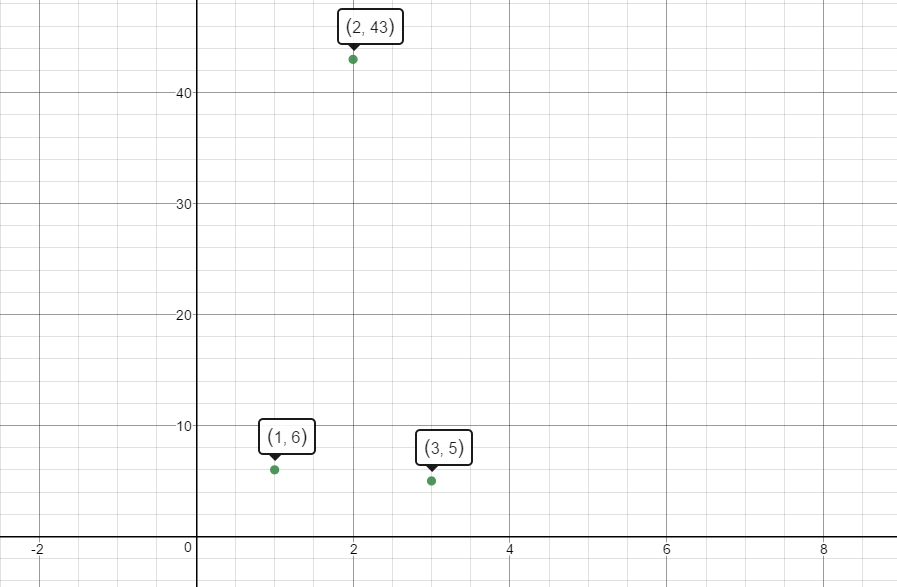
\includegraphics[width=13cm]{NewtonEj6} %hay que posicionar bien los gráficos
				\end{figure}	
			\end{itemize}
        \end{enumerate}
>>>>>>> 2d15196d83295c79463f3c1fbf4094e856e2e603
\end{enumerate}
\newpage
\section{Resolución de sistemas de ecuaciones no lineales:}
    
        
        En los siguientes ejercicios, use como criterio de parada lo siguiente:
        \begin{center}
            $ \frac{|| x^{n+1} - x^{n} ||}{|| x^{n+1} ||} \leq 10^{-6} $  
        \end{center}

        Donde $||z||=\sqrt{z_{1}^{2} + z_{2}^2+...+z_{n}^{2}} , z \in \mathbb{R}^{n}$
    \begin{enumerate}   
        
        \item Considere los siguientes sistemas de ecuaciones no lineales\\
        
        \begin{math}
            (a)\left\lbrace
          \begin{array}{ll}
                x^2 + xy^2-x-2&=0 \\\
                y^2 + xy^2-y+2&=0
            \end{array}
            \right.
            \hspace{3cm}
            (b) \left\lbrace
           \begin{array}{ll}
                 x^2+x-y^2&=1  \\
                 y-sen(x^2)&=0 
            \end{array}
            \right.
        \end{math}\\
        
        Usando el método de Newton, encuentre sus soluciones aproximadas. Para encontrar los puntos iniciales, apóyese en los gráficos que le permiten encontrar una aproximación de la solución 
        
        
        Pregunta $ 1a) $\\
        
            
            $ Recta(1) : x^2+xy^2-x-2=0 $
            
            $ Recta(2) : y^2 +xy^2-y+2=0 $
            
            \begin{figure}[h]
                \centering
                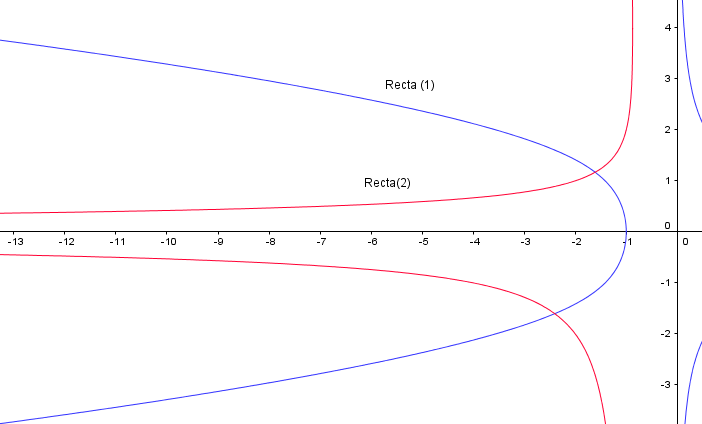
\includegraphics[width=15cm]{GraficoEcEj1a}
            \end{figure}
            
            Como se observa en el grafico las rectas (1) y (2) se intersectan 2 veces, mientras que su comportamiento luego tiende a alejarse una de la otra analizaremos las 2 soluciones que existen dentro de este intervalo de gráfica mostrado anteriormente.Posteriormente realizando un zoom en donde se encuentran las intersecciones se obtiene lo siguiente.\\
            
            \begin{figure}[H]
               \centering   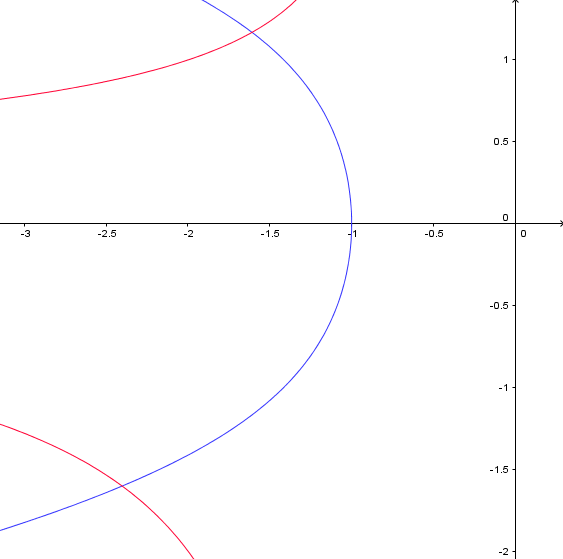
\includegraphics[width=13cm]{GraficoEcEj1azoom}
            \end{figure}
            Ahora para lograr obtener nuesta solucion que se encuentra en el 2do cuadrante  ocuparemos un punto cercano a la interseccion, En este caso ocuparemos $ x0=[-2;1] $ y el resulado obtenido como primera solución de la ecuación es :
            $ x*=[-1.6088;1.1686 ]$ siendo el punto  $x = -1.6088$,$y = 1.1686$
            
            Como ya obtuvimos la primera solución buscaremos la segunda, la cual se encuentra en el 3er cuadrante, para el cual igual usaremos un punto cercano a lo que se muestra en la gráfica como interseccion de las funciones.Por lo tanto ocuparemos el $x0=[-2;-1.8] $ obteniendo como el resultado el vector:
            $x*=[-2.4022;-1.6030]$ siendo el punto $x=-2.4022$, $y=-1.6030$

        \newpage    
        Pregunta $ 1b)$
        
            $ Recta(1) : x^2 + x -y^2=1 $
            
            $ Recta(2) : y-sen(x^2)=0  $
            
            \begin{figure}[h] \centering
            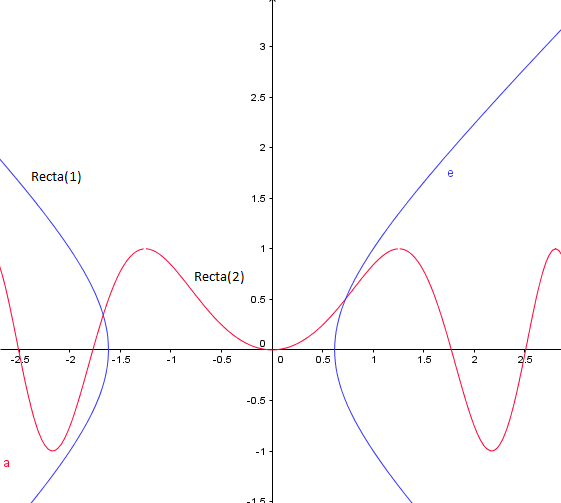
\includegraphics[width=12cm]{GraficoEcEj1b}
            \end{figure}
        Como se observa en la figura existen 2 soluciones del sistema no lineal, gracias a la gráfica dibujada dividiremos el problema en 2 casos, ocuparemos puntos cercanos a la intersección de las curvas dibujadas y asumiremos gracias a esta que no se intersectan en otro punto ya que  $ x \in (-inf,-2) \cup (1,inf+)$ las imagenes de las funciones se alejan.
        
        Con el error pedido en el inicio de este item el programa no logra terminar. debido a que el error es la condición de salida y que la diferencia  obtenida de una iteración con la otra nunca llega a ser tan pequeña como el intervalo a esperar. Para solucionar esto se redefine nuestra condición de salida por otra, en este caso se ocupo una cantidad de iteraciones igual a 5-6.
        
        Primero encontraremos la solución que se observa en el 1er cuadrante ,en este caso ocuparemos el punto inicial $x0 = [0.5;0.5]$ Obteniendo como solución el vector
        $ x*=[0.7272;0.5028] $ el punto $ x = 0.7272 $ , $ y = 0.5028$.
        
        Luego calcularemos la solución que en el gráfco se encuentra en el 2do cuadrante utilizando el punto inicial $0=[-1.8;0]$
        obteniendo como solución el vector $x*=[-1.6663;0.3612]$ el punto  $x=-1.6663$, $y=0.3612$

    
        \newpage
        
        \item En un sistema de tuberías (ver figura), los caudales de un cierto fluido en cada rama y las presiones en cada nodo de la red se relacionan mediante el siguiente sistema
        
        \begin{align*} 
            p1 - p2 &= KQ^{1,75} \\ 
            p2 - p4 &= K_1 Q_1^{1,75}\\
            p2 - p3 &= K_2 Q_2^{1,75}
        \end{align*}
        
    \begin{figure}[H]
    \centering
    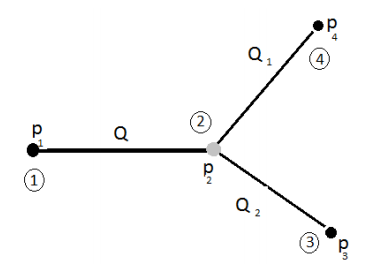
\includegraphics[width=7cm]{imagenEjec}
    \end{figure}        
    
    Para un determinado fluido se sabe que
    \begin{align*}
    p_1&=75psi & p_3&=20psi &  p_4&=15psi & K&=2,35e^{-3} & K_1&=4,67e^{-3} & K_2&=3,72e^{-2}
    \end{align*}
    
    Usando el método de Newton en varias variables, determine los caudales en todas las ramas, y la presión en el nodo 2 suponiendo que $Q = Q_1 + Q_2 $. Use como valores iniciales: $ p_2^0= 50 psi,$  $Q_2^0=7$ y  $Q_1^0=16$
    
    
    Reescribiendo las ecuaciones con valores dados:
    
    \begin{align*} 
        75 - p2 &=  2.35e^{-3}(Q_1+Q_2)^{1.75} \\ 
        p2 - 15 &= 4.67e^{-3}Q_1^{1.75} \\
        p2 - 20 &= 4.72e^{-2}Q_2^{1.75}
    \end{align*}
    
    Escribimos vector de funciones de la forma $f(x) = 0$

   $$\begin{pmatrix}
        75 - p2 - 2.35e^{-3}(Q_1+Q_2)^{1.75} &= 0 \\
        \\
        p2 - 15 - 4.67e^{-3}Q_1^{1.75} &= 0  \\
        \\
        p2 - 20 - 4.72e^{-2}Q_2^{1.75} &= 0
    \end{pmatrix}$$
    
    Utilizando los valores iniciales Se llega al resultado de : 
    $$\begin{pmatrix}
        p_2 &=44.5717 \hspace{0.1cm} psi \\
        \\
        Q_1 &=15.9418 \\
        \\
        Q_2 &=8.0495
    \end{pmatrix}$$
    Por lo tanto como $Q = Q_1 + Q_2 $ implica que $ Q = 23.9913 $
    
    Al igual que el ejercicio 1b) de éste item para lograr el objetivo de encontrar una raiz se limita a una cantidad de iteraciones iguales a 3, logrando así valores cercanos a la solución de la ecuación
    
    Para realizar este item se utilizo el código de NewtonVariables.m
    \end{enumerate}
    
\end{document}
